%-----------------------------------------------------------------------------
% Author: Ramsey (Rayla) Phuc
% Alias: Rayla Kurosaki
% GitHub: https://github.com/rkp1503
%-----------------------------------------------------------------------------
\documentclass{rayla-thesis-dissertation}
\usepackage{rayla-math-style}

%-----------------------------------------------------------------------------
% Project Information
%-----------------------------------------------------------------------------
\myUniversity{Rochester Institute of Technology}
\myCollege{College of Science}
\myDepartment{School of Mathematical and Statistics}
\myLogo{rit_logo.png}
% \myLogo{logo.eps}
\myTitle{Complex Dynamics of a Three Species Ecosystem}
\myName{Ramsey (Rayla) Phuc}
\myAdvisor{Dr. Ephraim Agyingi}
\submissionDate{\today}

%----------------------------------------------------------------------------- 
% Start of Document
%-----------------------------------------------------------------------------
\begin{document}

    \maketitle

    \newpage
    \tableofcontents

    %-------------------------------------------------------------------------
    % Abstract
    %-------------------------------------------------------------------------
    \begin{abstract}
        This paper investigates the dynamics of a model system by modifying key assumptions to explore alternative ecological interactions. The original model, outlined in the paper \cite{PANJA2022100153}, initially assumes a competition interaction between species $X$ and $Y$. However, we consider the implications of assuming a mutualism interaction instead. Additionally, we modify the assumption of a commensalism interaction between species $X$ and $Z$ to examine the consequences of an amensalism interaction. Furthermore, the model is expanded by assuming a logistic growth pattern for species Z. Through these modifications, we determine the new equilibrium points and conduct a comprehensive analysis of their characteristics. Numerical computations are performed to assess the stability or instability of the newly derived equilibrium points. The obtained results offer valuable insights into the dynamics and stability of the modified model, shedding light on the consequences of mutualism and amensalism interactions in the examined ecological system. This research contributes to a deeper understanding of the interrelationships between species interactions and population dynamics in ecological systems.
    \end{abstract}

    %-------------------------------------------------------------------------
    % Body
    %-------------------------------------------------------------------------
    % \tableofcontents
    % \section{Introduction}

    % \section{Original Model}

    % \section{Model 1}
    % \subsection{Constructing the Model}
    % \subsubsection{Model Properties}
    % \subsubsection{Property 1: Nonnegative solutions for nonnegative initial conditions}
    % \subsubsection{Property 2: Uniformly bounded}
    % \subsubsection{Property 3: Survival condition for Species Z}
    % \subsection{Analysis}
    % \subsubsection{Kolmogorov Analysis}
    % \subsubsection{Local Stability Analysis}
    % \subsubsection{Transcritical Bifurcation}
    % \subsubsection{Persistence of the System}
    % \subsection{Numerical Simulation}

    % \section{Model 2}
    % \subsection{Constructing the Model}
    % \subsection{Positivity and Boundedness of Solutions}
    % \subsection{Equilibrium Points and  Stability Analysis}
    % \subsubsection{Equilibrium Points}
    % \subsubsection{Local Stability Analysis}
    % \subsection{Hopf Bifurcation}
    % \subsubsection{Stability and Direction}

    % \section{Proposed/Modified Model}
    % \subsection{Constructing the Model}
    % \subsubsection{New/Modified Assumptions}
    % \subsubsection{Model Properties}
    % \subsubsection{Property 1: Nonnegative solutions for nonnegative initial conditions?}
    % \subsubsection{Property 2: Uniformly bounded?}
    % \subsubsection{Property 3: Survival condition for Species Z?}

    % \section{The Existance of Equilibria}

    % \section{Limit Cycle Analysis}

    % \section{Bifurcation Analysis of Identified Equilibria}

    % \section{Stability Analysis}
    % \subsection{Local Stability}
    % \subsection{Global Stability}

    % \section{Numerical Analysis and Simulations}

    % ----------------------------------------------------------------------------
% Author: Rayla Kurosaki
% GitHub: https://github.com/rkp1503
% ----------------------------------------------------------------------------

\section{Introduction}\label{sec:introduction}
In the vast realm of biological sciences, understanding the complex interplay of various phenomena is a formidable challenge. Nature's intricacies often defy direct observation and experimentation, necessitating the development of powerful tools that can unravel its hidden patterns. Enter mathematical models, a transformative approach that harnesses the language of mathematics to dissect, analyze, and predict the behavior of biological systems. These models serve as indispensable bridges between theoretical abstractions and empirical realities, enabling scientists to gain deeper insights into the fundamental principles that govern living organisms. By quantifying and formalizing biological processes, mathematical models offer a systematic framework to study intricate dynamics, investigate the consequences of different hypotheses, and guide experimental design.

There have been a plethora of models created to analyze the dynamics of such ecosystems. There are models which considers two species~\cite{GHOSH2017110, CHEN20122790, YU2012208167, HUANG2006672, AZIZALAOUI20031069, XIAO200614, SEN201212, CANTRELL2001206, CHEN20092905, CHEN2010246, KAR2005681, CHATTOPADHYAY1996287, KAR2003125}, three species~\cite{GAKKHAR201654, PANJA2022100153, MENG2014810, ALIDOUSTI2020109688, PEET2005491, SARWARDI2012133, PRIYADARSHI20133202, GAKKHAR2005105, GAKKHAR2007808, Mukherjee2013, DHAKNEMUNDE2012, CHATTOPADHYAY200345, PANJAMONDAL2015, PANJA2017389, KHAJANCHI2017193, JANA2017350} and four species~\cite{JANA2021100942}. Some of these models incorporate a functional response in their model, which include the Beddington–DeAngelis functional response~\cite{CANTRELL2001206}, the Crowley–Martin type functional response~\cite{MENG2014810}, the Holling-type I functional response~\cite{JANA2021100942, Mukherjee2013, CHATTOPADHYAY200345}, the Holling-type II functional response~\cite{GAKKHAR201654, PANJA2022100153, JANA2021100942, GHOSH2017110, YU2012208167, HUANG2006672, AZIZALAOUI20031069, CHEN2010246, SARWARDI2012133, PRIYADARSHI20133202, GAKKHAR2005105, GAKKHAR2007808, Mukherjee2013, CHATTOPADHYAY200345, PANJAMONDAL2015, JANA2017350}, the Holling-type III functional response~\cite{CHATTOPADHYAY200345}, the Leslie-Gower functional response~\cite{YU2012208167, AZIZALAOUI20031069, PRIYADARSHI20133202}, the Monod-Haldane type functional response~\cite{ALIDOUSTI2020109688}, and the Ratio-dependent functional response~\cite{XIAO200614, SEN201212, CANTRELL2001206, KHAJANCHI2017193}. Some models consider prey refuge~\cite{GAKKHAR201654, PANJA2022100153, GHOSH2017110, CHEN20122790, HUANG2006672, CHEN20092905, CHEN2010246, KAR2005681, SARWARDI2012133, Mukherjee2013, KHAJANCHI2017193, JANA2017350}, harvesting~\cite{XIAO200614, KAR2003125, PANJA2017389}, and the Allee effect~\cite{SEN201212}.

In this paper, we will consider a biological system that involves three species with each pairing of species have a unique interaction. In particular, we will study an ecosystem which involves predation, non-linear mutualism, and amensalism. The pairing of species that are in a predation interaction incorporates the Holling type II functional response and refuge into consideration.
    \section{Original Model}\label{sec:original_model}
In this section, we will go over the model that was featured in the paper written by Panja, Gayen, Kar, and Jana~\cite{PANJA2022100153}. The authors wanted to build a model of three species $X$, $Y$, $Z$ which contains three different types of species interactions. Namely nonlinear competition, predation, and commensalism.

\subsection{Assumptions on species $X$}\label{subsec:assumptions_x}
The authors have assumed that $X$ grows logistically at a rate of $r_x$ with a maximum capacity of $K_x$. The authors assumed that $X$ and $Y$ have a competition interaction with an interspecies competition coefficient $\alpha_{xy}$. The authors have also assumed that $X$ and $Z$ are in a commensalism interaction where $Z$ is a host of $X$ with a commensal coefficient $\delta$. From this, the authors have created the differential equation to represent the population of $X$:
\begin{equation}
    \diff[]{X}{T} = r_xX-\frac{r_x}{K_x}X^2-\frac{r_x\alpha_{xy}}{K_x}XY^2+\delta XZ
    \label{eq:2.1}
\end{equation}

\subsection{Assumptions on species $Y$}\label{subsec:assumptions_y}
The authors have assumed that $Y$ grows logistically at a rate of $r_y$ with a maximum capacity of $K_y$. The authors assumed that $Y$ and $X$ have a competition interaction with an interspecies competition coefficient $\alpha_{yx}$. The authors have also assumed that $Y$ and $Z$ are in a predation interaction where $Z$ preys on $Y$ via the Holling type II functional response with a half saturation constant $b$. $Z$ attacks $Y$ at a rate of $a$. Furthermore, as a result of being the prey to $Z$, $Y$ shows refuge behavior with a refuge rate of $p$. From this, the authors have created the differential equation to represent the population of $Y$:
\begin{equation}
    \diff[]{Y}{T} = r_yY-\frac{r_y}{K_y}Y^2-\frac{r_y\alpha_{yx}}{K_y}X^2Y-\frac{a\left(1-p\right)YZ}{b+\left(1-p\right)Y}
    \label{eq:2.2}
\end{equation}

\subsection{Assumptions on species $Z$}\label{subsec:assumptions_z}
The authors assumed that $Z$ grows as a result of being in a predation interaction with $Y$ via the Holling type II functional response with a half saturation constant $b$ and $c$ as the conservation rate of $Y$. Furthermore, the authors assume that the population of $Z$ decays at a rate of $e$. From this, the authors have created the differential equation to represent the population of $Z$:
\begin{equation}
    \diff[]{Z}{T} = \frac{ac\left(1-p\right)YZ}{b+\left(1-p\right)Y}-eZ
    \label{eq:2.3}
\end{equation}

\subsection{Building the model}\label{subsec:model}
From the assumptions, the governing equations for this model are:
\begin{subequations}
    \begin{align}
        \diff[]{X}{T} &= r_xX-\frac{r_x}{K_x}X^2-\frac{r_x\alpha_{xy}}{K_x}XY^2+\delta XZ
        \label{model:2.1a}\\
        \diff[]{Y}{T} &= r_yY-\frac{r_y}{K_y}Y^2-\frac{r_y\alpha_{yx}}{K_y}X^2Y-\frac{a\left(1-p\right)YZ}{b+\left(1-p\right)Y}
        \label{model:2.b}\\
        \diff[]{Z}{T} &= \frac{ac\left(1-p\right)YZ}{b+\left(1-p\right)Y}-eZ
        \label{model:2.1c}
    \end{align}
    \label{model:2.1}
\end{subequations}
and with the following substitutions:
\begin{gather*}
    T=\frac{t}{r_x},\ X=K_xx,\ Y=K_yy,\ Z=\frac{r_xK_y}{a}z\\
    \alpha_{xy}=\frac{K_x}{K_y^2}\gamma_{12},\ \alpha_{yx}=\frac{K_y}{K_x^2}\gamma_{21},\ \delta=\frac{a}{K_y}\gamma\\
    r=\frac{r_y}{r_x},\ b=K_yv_1,\ e=r_xv_2,\ c=\frac{r_xv_3}{a}\\
\end{gather*}
the authors have simplified and non-dimensionalized \myref[Model]{model:2.1}. This gives us the following model the authors have used throughout their paper:
\begin{subequations}
    \begin{align}
        \diff[]{x}{t} &= x\left(1-x-\gamma_{12}y^2\right)+\gamma xz
        \label{model:2.2a}\\
        \diff[]{y}{t} &= ry\left(1-y-\gamma_{21}x^2\right)-\frac{\left(1-p\right)yz}{v_1+\left(1-p\right)y}
        \label{model:2.2b}\\
        \diff[]{z}{t} &= z\left(\frac{v_3\left(1-p\right)y}{v_1+\left(1-p\right)y}-v_2\right)
        \label{model:2.2c}
    \end{align}
    \label{model:2.2}
\end{subequations}
    \section{Revised/Modified Model}\label{sec:modified_model}
In \myref[Section]{sec:original_model}, we discussed the model the authors used in their paper and the assumptions that were used to construct it. In this section, we will modify some of the initial assumptions that the authors have made when creating their model to obtain a new model that we will analyze throughout this paper.

\subsection{Modification 1: The interaction between species $X$ and $Y$}\label{subsec:modification_1}
The original model assumes that species $X$ and $Y$ are in a competition interaction. Instead of considering an interaction that negatively impacts both species, lets consider an interaction that benefits both species. Thus, we will assume that species $X$ and $Y$ are in a mutualism interaction.

\subsection{Modification 2: The interaction between species $X$ and $Z$}\label{subsec:modification_2}
The original model assumes that species $X$ and $Z$ are in a commensalism interaction where species $X$ is benefiting from species $Z$. Instead of considering an interaction where species $X$ gets positively impacted, lets consider an interaction where species $X$ gets negatively impacted while being in an interaction with species $Z$. Thus, we will assume that species $X$ and $Z$ are in an amensalism interaction.

\subsection{Modification 3: The growth rate of species $Z$}\label{subsec:modification_3}
The original model assumes that species $Z$ grows solely due to being in a predation interaction with species $Y$. Here, we will assume that species $Z$ not only grows due to being in a predation interaction with species $Y$, but also grows logistically with a rate of $r_z$ with a capacity of $K_z$.

\subsection{Building the modified model}\label{subsec:modified_model}
With these modified assumptions, the authors' original model become:
\begin{subequations}
    \begin{align}
        \diff[]{X}{T} &= r_xX-\frac{r_x}{K_x}X^2+\frac{r_x\alpha_{xy}}{K_x}XY^2-\delta XZ
        \label{model:3.1a}\\
        \diff[]{Y}{T} &= r_yY-\frac{r_y}{K_y}Y^2+\frac{r_y\alpha_{yx}}{K_y}X^2Y-\frac{a\left(1-p\right)YZ}{b+\left(1-p\right)Y}
        \label{model:3.1b}\\
        \diff[]{Z}{T} &= r_zZ-\frac{r_z}{K_z}Z^2+\frac{ac\left(1-p\right)YZ}{b+\left(1-p\right)Y}-eZ
        \label{model:3.1c}
    \end{align}
    \label{model:3.1}
\end{subequations}
and with the following substitutions:
\begin{gather*}
    X=K_xx,\ Y=K_yy,\ Z=\frac{r_xK_y}{a}z,\ T=\frac{1}{r_x}t\\
    r_1=\frac{r_y}{r_x},\ r_2=\frac{r_z}{r_x},\ v_1=\frac{b}{K_y},\ v_2=\frac{e}{r_x},\ v_3=\frac{ac}{r_x}\\
    \gamma_{12}=\frac{\alpha_{xy}K_y^2}{K_x},\ \gamma_{21}=\frac{\alpha_{yx}K_x^2}{K_y},\ \gamma_{13}=\frac{\delta K_y}{a},\ \gamma_{31}=\frac{r_xK_y}{aK_z}\\
\end{gather*}
we can simplify and non-dimensionalize \myref[Model]{model:3.1}. This gives us the following model we will work on throughout this paper:
\begin{subequations}
    \begin{align}
        \diff[]{x}{t} &= x\left(1-x+\gamma_{12}y^2\right)-\gamma_{13}xz
        \label{model:3.2a}\\
        \diff[]{y}{t} &= r_1y\left(1-y+\gamma_{21}x^2\right)-\frac{\left(1-p\right)yz}{v_1+\left(1-p\right)y}
        \label{model:3.2b}\\
        \diff[]{z}{t} &= r_2z\left(1-\gamma_{31}z\right)+z\left(\frac{v_3\left(1-p\right)y}{v_1+\left(1-p\right)y}-v_2\right)
        \label{model:3.2c}
    \end{align}
    \label{model:3.2}
\end{subequations}

% \begin{table*}[b]
%     \centering
%     \begin{tabular}{l|l}\hline
%         Variable & Description \\ \hline
%         $X,Y$ & Densities of two logistically growing competing species.\\
%         $Z$ & Density of a species which preys on $Y$ ($Z$ eats $Y$)\\
%         $r_x,r_y$ & Intrinsic growth rate of species $X$ and $Y$ respectively\\
%         $\alpha_{12},\alpha_{21}$ & Inter-species competition between two species $X$ and $Y$ respectively\\
%         $a_x,a_y$ & Attack rate of species $Z$ on species $X$ and $Y$ respectively.\\
%         $p_x,p_y$ & Refuge rate of species $X$ and $Y$ respectively.\\
%         $c_x,c_y$ & Conservation rate of species $X$ and $Y$ respectively.\\
%         $b$ & Half saturation constant for Holling type II function.\\
%         $e$ & Death rate of $Z$ species.\\\hline
%     \end{tabular}
%     \caption{Caption}
%     \label{tab:3.1}
% \end{table*}

% \lipsum[1]

    \section{Identifying Equilibria}\label{sec:identify_equilibria}
In \myref[Section]{sec:modified_model}, we have modified some of the assumptions the authors have made and created \myref[Model]{model:3.2} based on the new/modified assumptions. In this section, we will find all the equilibria present in our model. To find all the equilibria $\left(x^*,y^*,z^*\right)$ of this system, we will set all the equations in \myref[Model]{model:3.1} equal to 0~\cite{book:2478639}.
\begin{subequations}
    \begin{align}
        0 &= x^*\left(1-x^*+\gamma_{12}\left(y^*\right)^2\right)-\gamma_{13}x^*z^*
        \label{eq:4.1a}\\
        0 &= r_1y^*\left(1-y^*+\gamma_{21}\left(x^*\right)^2\right)-\frac{\left(1-p\right)y^*z^*}{v_1+\left(1-p\right)y^*}
        \label{eq:4.1b}\\
        0 &= r_2z^*\left(1-\gamma_{31}z^*\right)+z^*\left(\frac{v_3\left(1-p\right)y^*}{v_1+\left(1-p\right)y^*}-v_2\right)
        \label{eq:4.1c}
    \end{align}
    \label{eq:4.1}
\end{subequations}

\subsection{Case 1: The trivial equilibrium}\label{subsec:trivial_equilibrium}
The trivial equilibrium is where $\left(x^*.y^*.z^*\right)=(0,0,0)$. To verify that the trivial equilibrium exists in \myref[Model]{model:3.2}, we will plug in $x^*=0$, $y^*=0$, and $z^*=0$ into the model and must conclude that each equation reduces to $0=0$. Plugging $x^*=0$, $y^*=0$, and $z^*=0$ into \myref[Model]{model:3.2} yields:
\begin{align*}
    0 &= (0)\left(1-(0)+\gamma_{12}(0)^2\right)-\gamma_{13}(0)(0)\\
    0 &= r_1(0)\left(1-(0)+\gamma_{21}(0)^2\right)-\frac{\left(1-p\right)(0)(0)}{v_1+\left(1-p\right)(0)}\\
    0 &= r_2(0)\left(1-\gamma_{31}(0)\right)+(0)\left(\frac{v_3\left(1-p\right)(0)}{v_1+\left(1-p\right)(0)}-v_2\right)
\end{align*}
By inspection, we can see that each equation reduces to $0=0$. Thus, we can say that the trivial equilibrium exists:
\[
\fbox{$\displaystyle E_0=\left(0,0,0\right)$}
\]

\subsection{Case 2: The $x$-axial equilibrium}\label{subsec:x_axial_equilibrium}
The $x$-axial equilibrium is an equilibrium where $x^*$ is non-zero and the other components of the equilibrium are 0. Since we are talking about population densities, it does not make sense to consider values of $x^*$ where $x^*<0$. Thus, the conditions to impose when finding the $x$-axial equilibrium are $x^*>0$ and all other components are 0. To find the $x$-axial equilibrium of \myref[Model]{model:3.2}, we will plug in $y^*=0$ and $z^*=0$:
\begin{align*}
    0 &= x^*\left(1-x^*+\gamma_{12}(0)^2\right)-\gamma_{13}x^*(0)\\
    0 &= r_1(0)\left(1-(0)+\gamma_{21}\left(x^*\right)^2\right)-\frac{\left(1-p\right)(0)(0)}{v_1+\left(1-p\right)(0)}\\
    0 &= r_2(0)\left(1-\gamma_{31}(0)\right)+(0)\left(\frac{v_3\left(1-p\right)(0)}{v_1+\left(1-p\right)(0)}-v_2\right)
\end{align*}
which reduces to:
\begin{equation}
    0 = x^*\left(1-x^*\right)
    \label{eq:4.2}
\end{equation}
\myref[Equation]{eq:4.2} yields solutions $x^*=\left\{0, 1\right\}$. However, due the condition $x^*>0$ we imposed, the only valid solution to consider is $x^*=1$. With this value of $x^*$, we have concluded that the $x$-axial equilibrium exists:
\[
\fbox{$\displaystyle E_x=\left(
1,
0,
0
\right)$}
\]

\subsection{Case 3: The $y$-axial equilibrium}\label{subsec:y_axial_equilibrium}
The $y$-axial equilibrium is an equilibrium where $y^*$ is non-zero and the other components of the equilibrium are 0. Since we are talking about population densities, it does not make sense to consider values of $y^*$ where $y^*<0$. Thus, the conditions to impose when finding the $y$-axial equilibrium are $y^*>0$ and all other components are 0. To find the $y$-axial equilibrium of \myref[Model]{model:3.2}, we will plug in $x^*=0$ and $z^*=0$:
\begin{align*}
    0 &= (0)\left(1-(0)+\gamma_{12}\left(y^*\right)^2\right)-\gamma_{13}(0)(0)\\
    0 &= r_1y^*\left(1-y^*+\gamma_{21}(0)^20\right)-\frac{\left(1-p\right)y^*(0)}{v_1+\left(1-p\right)y^*}\\
    0 &= r_2(0)\left(1-\gamma_{31}(0)\right)+(0)\left(\frac{v_3\left(1-p\right)y^*}{v_1+\left(1-p\right)y^*}-v_2\right)
\end{align*}
which reduces to:
\begin{equation}
    r_1y^*\left(1-y^*\right)=0
    \label{eq:4.3}
\end{equation}
Since all parameters are positive, \myref[Equation]{eq:4.3} yields solutions $y^*=\left\{0, 1\right\}$. However, due the condition $y^*>0$ we imposed, the only valid solution to consider is $y^*=1$. With this value of $y^*$, we have concluded that the $y$-axial equilibrium exists:
\[
\fbox{$\displaystyle E_y=\left(
0,
1,
0
\right)$}
\]

\subsection{Case 4: The $z$-axial equilibrium}\label{subsec:z_axial_equilibrium}
The $z$-axial equilibrium is an equilibrium where $z^*$ is non-zero and the other components of the equilibrium are 0. Since we are talking about population densities, it does not make sense to consider values of $z^*$ where $z^*<0$. Thus, the conditions to impose when finding the $z$-axial equilibrium are $z^*>0$ and all other components are 0. To find the $z$-axial equilibrium of \myref[Model]{model:3.2}, we will plug in $x^*=0$ and $y^*=0$:
\begin{align*}
    0 &= (0)\left(1-(0)+\gamma_{12}(0)^2\right)-\gamma_{13}(0)z^*\\
    0 &= r_1(0)\left(1-(0)+\gamma_{21}(0)^2\right)-\frac{\left(1-p\right)(0)z^*}{v_1+\left(1-p\right)(0)}\\
    0 &= r_2z^*\left(1-\gamma_{31}z^*\right)+z^*\left(\frac{v_3\left(1-p\right)(0)}{v_1+\left(1-p\right)(0)}-v_2\right)
\end{align*}
which reduces to:
\begin{equation}
    r_2z^*\left(1-\gamma_{31}z^*\right)-v_2z^*=0
    \label{eq:4.4}
\end{equation}
Since all parameters are positive, \myref[Equation]{eq:4.3} yields solutions
\[
z^*=\left\{0, \frac{r_2-v_2}{\gamma_{31}r_2}\right\}
\]
However, due the condition $z^*>0$ we imposed, the only valid solution to consider is:
\[
z^*=\frac{r_2-v_2}{\gamma_{31}r_2}
\]
With this value of $z^*$, we have concluded that the $z$-axial equilibrium exists:
\[
\fbox{$\displaystyle E_z=\left(
0,
0,
\frac{r_2-v_2}{\gamma_{31}r_2}
\right)$}
\]
under the condition:
\[
r_2>v_2
\]

\subsection{Case 5: The $xy$-boundary equilibrium}\label{subsec:xy_boundary_equilibrium}
The $xy$-boundary equilibrium is an equilibrium where $x^*$ and $y^*$ are non-zero and all other components of the equilibrium are 0. Since we are talking about population densities, it does not make sense to consider values of $x^*$ and $y^*$ where $x^*<0$ and $y^*<0$. Thus, the conditions to impose when finding the $xy$-boundary equilibrium are $x^*>0$ and $y^*>0$ and all other components are 0. To find the $xy$-boundary equilibrium of \myref[Model]{model:3.2}, we will plug in $z^*=0$:
\begin{align*}
    0 &= x^*\left(1-x^*+\gamma_{12}\left(y^*\right)^2\right)-\gamma_{13}x^*(0)\\
    0 &= r_1y^*\left(1-y^*+\gamma_{21}\left(x^*\right)^2\right)-\frac{\left(1-p\right)y^*(0)}{v_1+\left(1-p\right)y^*}\\
    0 &= r_2(0)\left(1-\gamma_{31}(0)\right)+(0)\left(\frac{v_3\left(1-p\right)y^*}{v_1+\left(1-p\right)y^*}-v_2\right)
\end{align*}
which reduces to:
\begin{subequations}
    \begin{align}
        0 &= x^*\left(1-x^*+\gamma_{12}\left(y^*\right)^2\right)
        \label{eq:4.5a}\\
        0 &= r_1y^*\left(1-y^*+\gamma_{21}\left(x^*\right)^2\right)
        \label{eq:4.5b}
    \end{align}
    \label{eq:4.5}
\end{subequations}
With the conditions $x^*>0$ and $y^*>0$ we imposed, the \myref[System]{eq:4.5} reduces to:
\begin{subequations}
    \begin{align}
        0 &= 1-x^*+\gamma_{12}\left(y^*\right)^2
        \label{eq:4.6a}\\
        0 &= 1-y^*+\gamma_{21}\left(x^*\right)^2
        \label{eq:4.6b}
    \end{align}
    \label{eq:4.6}
\end{subequations}
We can solve for $x^*$ in \myref[Equation]{eq:4.6a}:
\begin{equation}
    x^*=1+\gamma_{12}\left(y^*\right)^2
    \label{eq:4.7}
\end{equation}
and plug \myref[Equation]{eq:4.7} into \myref[Equation]{eq:4.6b} to get:
\begin{equation}
    \gamma_{12}^2\gamma_{21}\left(y^*\right)^4+2\gamma_{12}\gamma_{21}\left(y^*\right)^2-y^*+\left(\gamma_{21}+1\right)=0
    \label{eq:4.8}
\end{equation}
There isn't a nice closed-form solution to \myref[Equation]{eq:4.8} so we will show that there exist a $y^*$ such that \myref[Equation]{eq:4.8} is satisfied. To do this, we will use the intermediate value theorem~\cite{book:2946356}. Let
\[
f\left(y^*\right)=\gamma_{12}^2\gamma_{21}\left(y^*\right)^4+2\gamma_{12}\gamma_{21}\left(y^*\right)^2-y^*+\left(\gamma_{21}+1\right)
\]
Here, we can see that $f(0)=\gamma_{21}+1$. Since all parameters are positive, this means that $f(0)>0$. Let $f(\beta)<0$ for some value of $\beta$. $f\left(\beta\right)<0$ implies:
\[
\gamma_{12}<\frac1{\beta^2}\left(\sqrt{\frac{\beta-1}{\gamma_{21}}}-1\right)
\]
Therefore we can say that the $xy$-boundary equilibrium $E_{xy}=\left(\hat{x},\hat{y},0\right)$ exists where
\[
\hat{x}=1+\gamma_{12}\left(\hat{y}\right)^2
\]
and $y^*$ is a positive solution to the equation:
\[
\gamma_{12}^2\gamma_{21}\left(\hat{y}\right)^4+2\gamma_{12}\gamma_{21}\left(\hat{y}\right)^2-\hat{y}+\gamma_{21}+1=0
\]
if the following condition is satisfied for some value of $\beta>0$:
\[
\gamma_{12}<\frac1{\beta^2}\left(\sqrt{\frac{\beta-1}{\gamma_{21}}}-1\right)
\]

\subsection{Case 6: The $xz$-boundary equilibrium}\label{subsec:xz_boundary_equilibrium}
The $xz$-boundary equilibrium is an equilibrium where $x^*$ and $z^*$ are non-zero and all other components of the equilibrium are 0. Since we are talking about population densities, it does not make sense to consider values of $x^*$ and $z^*$ where $x^*<0$ and $z^*<0$. Thus, the conditions to impose when finding the $xz$-boundary equilibrium are $x^*>0$ and $z^*>0$ and all other components are 0. To find the $xz$-boundary equilibrium of \myref[Model]{model:3.2}, we will plug in $y^*=0$:
\begin{align*}
    0 &= x^*\left(1-x^*+\gamma_{12}(0)^2\right)-\gamma_{13}x^*z^*\\
    0 &= r_1(0)\left(1-(0)+\gamma_{21}\left(x^*\right)^2\right)-\frac{\left(1-p\right)(0)z^*}{v_1+\left(1-p\right)(0)}\\
    0 &= r_2z^*\left(1-\gamma_{31}z^*\right)+z^*\left(\frac{v_3\left(1-p\right)(0)}{v_1+\left(1-p\right)(0)}-v_2\right)
\end{align*}
which reduces to:
\begin{subequations}
    \begin{align}
        0 &= x^*\left(1-x^*\right)-\gamma_{13}x^*z^*
        \label{eq:4.9a}\\
        0 &= r_2z^*\left(1-\gamma_{31}z^*\right)-v_2z^*
        \label{eq:4.9b}
    \end{align}
    \label{eq:4.9}
\end{subequations}
With the conditions $x^*>0$ and $z^*>0$ we imposed, the \myref[System]{eq:4.9} reduces to:
\begin{subequations}
    \begin{align}
        0 &= 1-x^*-\gamma_{13}z^*
        \label{eq:4.10a}\\
        0 &= r_2\left(1-\gamma_{31}z^*\right)-v_2
        \label{eq:4.10b}
    \end{align}
    \label{eq:4.10}
\end{subequations}
We can solve for $z^*$ in \myref[Equation]{eq:4.10b}:
\begin{equation}
    z^*=\frac{r_2-v_2}{\gamma_{31}r_2}
    \label{eq:4.11}
\end{equation}
To ensure that $z^*>0$, we need to impose the condition $r_2>v_2$. Plugging \myref[Equation]{eq:4.11} into \myref[Equation]{eq:4.10a}, we get:
\begin{equation}
    1-x^*-\gamma_{13}\left(\frac{r_2-v_2}{\gamma_{31}r_2}\right)=0
    \label{eq:4.12}
\end{equation}
Solving for $x^*$ in \myref[Equation]{eq:4.12}, we get:
\begin{equation}
    x^*=1-\frac{\gamma_{13}\left(r_2-v_2\right)}{\gamma_{31}r_2}
    \label{eq:4.13}
\end{equation}
To ensure that $x^*>0$, we need to impose the condition
\[
\frac{\gamma_{31}r_2}{\gamma_{13}}>0
\]
With \myref[Equation]{eq:4.13}, $y^*=0$, and \myref[Equation]{eq:4.11}, we can conclude that the $xz$-boundary equilibrium exists:
\[
\fbox{$\displaystyle E_{xz}=\left(
1-\frac{\gamma_{13}\left(r_2-v_2\right)}{\gamma_{31}r_2},
0,
\frac{r_2-v_2}{\gamma_{31}r_2}
\right)$}
\]
under the conditions:
\[
r_2>v_2,\quad \frac{\gamma_{31}r_2}{\gamma_{13}}>0
\]

\subsection{Case 7: The $yz$-boundary equilibrium}\label{subsec:yz_boundary_equilibrium}
The $yz$-boundary equilibrium is an equilibrium where $y^*$ and $z^*$ are non-zero and all other components of the equilibrium are 0. Since we are talking about population densities, it does not make sense to consider values of $y^*$ and $z^*$ where $y^*<0$ and $z^*<0$. Thus, the conditions to impose when finding the $yz$-boundary equilibrium are $y^*>0$ and $z^*>0$ and all other components are 0. To find the $yz$-boundary equilibrium of \myref[Model]{model:3.2}, we will plug in $x^*=0$:
\begin{align*}
    0 &= (0)\left(1-(0)+\gamma_{12}\left(y^*\right)^2\right)-\gamma_{13}(0)z^*\\
    0 &= r_1y^*\left(1-y^*+\gamma_{21}(0)^2\right)-\frac{\left(1-p\right)y^*z^*}{v_1+\left(1-p\right)y^*}\\
    0 &= r_2z^*\left(1-\gamma_{31}z^*\right)+z^*\left(\frac{v_3\left(1-p\right)y^*}{v_1+\left(1-p\right)y^*}-v_2\right)
\end{align*}
which reduces to:
\begin{subequations}
    \begin{align}
        0 &= r_1y^*\left(1-y^*\right)-\frac{\left(1-p\right)y^*z^*}{v_1+\left(1-p\right)y^*}
        \label{eq:4.14a}\\
        0 &= r_2z^*\left(1-\gamma_{31}z^*\right)+z^*\left(\frac{v_3\left(1-p\right)y^*}{v_1+\left(1-p\right)y^*}-v_2\right)
        \label{eq:4.14b}
    \end{align}
    \label{eq:4.14}
\end{subequations}
With the conditions $y^*>0$ and $z^*>0$ we imposed, the \myref[System]{eq:4.14} reduces to:
\begin{subequations}
    \begin{align}
        0 &= r_1\left(1-y^*\right)-\frac{\left(1-p\right)z^*}{v_1+\left(1-p\right)y^*}
        \label{eq:4.15a}\\
        0 &= r_2\left(1-\gamma_{31}z^*\right)+\left(\frac{v_3\left(1-p\right)y^*}{v_1+\left(1-p\right)y^*}-v_2\right)
        \label{eq:4.15b}
    \end{align}
    \label{eq:4.15}
\end{subequations}
We can solve for $z^*$ in \myref[Equation]{eq:4.15b}:
\begin{equation}
    z^*=\frac{r_2-v_2}{\gamma_{31}r_2}+\frac{v_3\left(1-p\right)y^*}{\gamma_{31}r_2\left(v_1+\left(1-p\right)y^*\right)}
    \label{eq:4.16}
\end{equation}
To ensure that $z^*>0$, we need to impose the condition $r_2>v_2$. To solve for $y^*$, we will plug in \myref[Equation]{eq:4.16} into \myref[Equation]{eq:4.15a} to get the equation:
\begin{equation}
    \frac{Y_3\left(y^*\right)^3+Y_2\left(y^*\right)^2+Y_1y^*+Y_0}{\gamma_{31}r_2\left(v_1+\left(1-p\right)y^*\right)^2}=0
    \label{eq:4.17}
\end{equation}
where
\begin{align*}
    Y_3 &= -\gamma_{31}r_1r_2\left(1-p\right)^2\\
    Y_2 &= \gamma_{31}r_1r_2\left(\left(1-p\right)-2v_1\right)\left(1-p\right)\\
    Y_1 &= \gamma_{31}r_1r_2v_1\left(2\left(1-p\right)-v_1\right)+\left(v_2-v_3-r_2\right)\left(1-p\right)^2\\
    Y_0 &= \gamma_{31}r_1r_2v_1^2+v_1\left(v_2-r_2\right)\left(1-p\right)
\end{align*}
Note that we can eliminate one value of $y^*$ form \myref[Equation]{eq:4.17}:
\[
\left(v_1+\left(1-p\right)y^*\right)^2\neq0 \implies y^*\neq-\frac{v_1}{1-p}
\]
and simplify \myref[Equation]{eq:4.17} to:
\begin{equation}
    Y_3\left(y^*\right)^3+Y_2\left(y^*\right)^2+Y_1y^*+Y_0=0
    \label{eq:4.18}
\end{equation}
With a third degree polynomial with complex coefficients, it will be difficult to derive the closed-form solutions to \myref[Equation]{eq:4.18}. However, we don't need to find the exact form of the $y^*$ component in this equilibrium. It is sufficient to show that a positive solution to \myref[Equation]{eq:4.18} exists. This is because if $y^*=0$, then it will lead to the $z$-axial equilibrium and if $y^*<0$ or if $y^*$ is complex, then we ignore it since it biologically does not make sense. Going through the coefficients of \myref[Equation]{eq:4.18}, we can immediately see that $Y_3<0$. For $Y_2$, we can place a condition to determine when its positive or negative. In particular, we can say that
\[
\begin{dcases}
    Y_2<0 &\text{if}\quad 1-p<2v_1\\
    Y_2>0 &\text{if}\quad 1-p>2v_1
\end{dcases}
\]
For $Y_1$, we have:
\[
\begin{dcases}
    Y_1<0 &\text{if}\quad \frac{\gamma_{31}r_1r_2v_1\left(2\left(1-p\right)-v_1\right)}{\left(r_2-v_2+v_3\right)\left(1-p\right)^2}<1\\
    Y_1>0 &\text{if}\quad \frac{\gamma_{31}r_1r_2v_1\left(2\left(1-p\right)-v_1\right)}{\left(r_2-v_2+v_3\right)\left(1-p\right)^2}>1
\end{dcases}
\]
and for $Y_0$, we have:
\[
\begin{dcases}
    Y_0<0 &\text{if}\quad \frac{\gamma_{31}r_1r_2v_1}{\left(r_2-v_2\right)\left(1-p\right)}<1\\
    Y_0>0 &\text{if}\quad \frac{\gamma_{31}r_1r_2v_1}{\left(r_2-v_2\right)\left(1-p\right)}>1
\end{dcases}
\]
Note that we had to impose a condition on $z^*$, which was $r_2>v_2$. With this condition, we can rewrite one our conditions on $Y_0$:
\[
\begin{dcases}
    Y_0<0 &\text{if}\quad \frac{\gamma_{31}r_1r_2v_1}{1-p}<r_2-v_2\\
    Y_0>0 &\text{if}\quad \frac{\gamma_{31}r_1r_2v_1}{1-p}>0
\end{dcases}
\]
and for $Y_1$, the conditions can be rewritten as:
\[
\begin{dcases}
    Y_1<0 &\text{if}\quad \frac{\gamma_{31}r_1r_2v_1\left(2\left(1-p\right)-v_1\right)}{\left(1-p\right)^2}<r_2-v_2+v_3\\
    Y_1>0 &\text{if}\quad 1-p>\frac{v_1}2
\end{dcases}
\]
By Descartes' rule of signs~\cite{10.2307/1967494}, we can say that \myref[Equation]{eq:4.18} has at least one positive solution if $Y_3<0$ and $Y_2,Y_1,Y_0>0$. This means that we must impose the conditions:
\[
1-p>2v_1,\quad 1-p>\frac{v_1}2,\quad \frac{\gamma_{31}r_1r_2v_1}{1-p}>0
\]
Since all parameters are positive, the third condition is always fulfilled. Also, we know that $2v_1>v_1/2$ so the second condition is redundant. Therefore, we can say that the $yz$-boundary equilibrium $E_{yz}=\left(0,\bar{y},\bar{z}\right)$ exists where:
\[
\bar{z}=\frac{r_2-v_2}{\gamma_{31}r_2}+\frac{v_3\left(1-p\right)\bar{y}}{\gamma_{31}r_2\left(v_1+\left(1-p\right)\bar{y}\right)}
\]
with a condition that $r_2>v_2$ and $\bar{y}$ is a positive root to the equation:
\begin{equation*}
    Y_3\left(\bar{y}\right)^3+Y_2\left(\bar{y}\right)^2+Y_1\bar{y}+Y_0=0
\end{equation*}
where
\begin{align*}
    Y_3 &= -\gamma_{31}r_1r_2\left(1-p\right)^2\\
    Y_2 &= \gamma_{31}r_1r_2\left(\left(1-p\right)-2v_1\right)\left(1-p\right)\\
    Y_1 &= \gamma_{31}r_1r_2v_1\left(2\left(1-p\right)-v_1\right)+\left(v_2-v_3-r_2\right)\left(1-p\right)^2\\
    Y_0 &= \gamma_{31}r_1r_2v_1^2+v_1\left(v_2-r_2\right)\left(1-p\right)
\end{align*}
with a condition that $1-p>2v_1$.

\subsection{Case 8: The interior equilibrium}\label{subsec:interior_equilibrium}
The interior equilibrium is an equilibrium where all the components of the equilibrium are non-zero. Since we are talking about population densities, having non-zero components that are also negative would not make sense. Thus, the conditions to impose when finding the interior equilibrium are when the components are positive. To find the interior equilibrium of \myref[Model]{model:3.2}, we know that $x^*,y^*,z^*\neq0$. So we can reduce the model to:
\begin{subequations}
    \begin{align}
        0 &= 1-x^*+\gamma_{12}\left(y^*\right)^2-\gamma_{13}z^*
        \label{eq:4.21a}\\
        0 &= r_1\left(1-y^*+\gamma_{21}\left(x^*\right)^2\right)-\frac{\left(1-p\right)z^*}{v_1+\left(1-p\right)y^*}
        \label{eq:4.21b}\\
        0 &= r_2\left(1-\gamma_{31}z^*\right)+\left(\frac{v_3\left(1-p\right)y^*}{v_1+\left(1-p\right)y^*}-v_2\right)
        \label{eq:4.21c}
    \end{align}
    \label{eq:4.21}
\end{subequations}
We can solve for $x^*$ in \myref[Equation]{eq:4.21a}:
\begin{equation}
    x^*=1+\gamma_{12}\left(y^*\right)^2-\gamma_{13}z^*
    \label{eq:4.22}
\end{equation}
To ensure that $x^*>0$, we will need to impose the condition:
\[
z^*<\frac{1+\gamma_{12}\left(y^*\right)^2}{\gamma_{13}}
\]
We can also solve for $z^*$ in \myref[Equation]{eq:4.21c}:
\begin{equation}
    z^*=\frac{r_2-v_2}{\gamma_{31}r_2}+\frac{v_3\left(1-p\right)y^*}{\gamma_{31}r_2\left(v_1+\left(1-p\right)y^*\right)}
    \label{eq:4.23}
\end{equation}
To ensure that $z^*>0$, we will need to impose the condition $r_2>v_2$. With \myref[Equation]{eq:4.22} and \myref[Equation]{eq:4.23}, we can plug them into \myref[Equation]{eq:4.21b} to obtain the following Equation:
\begin{equation}
    \frac{1}{\gamma_{13}^2r_2^2\left(v_1+\left(1-p\right)y^*\right)^2}\sum_{i=0}^6 Y_i\left(y^*\right)^i=0
    \label{eq:4.24}
\end{equation}
where
\begin{align*}
    Y_6 &= \gamma_{12}^2\gamma_{21}\gamma_{31}^2r_1r_2^2\left(1-p\right)^2\\
    Y_5 &= 2\gamma_{12}^2\gamma_{21}\gamma_{31}^2r_1r_2^2v_1\left(1-p\right)\\
    Y_4 &= \gamma_{12}\gamma_{21}\gamma_{31}r_1r_2\left(2\gamma_{13}\left(v_2-r_2-v_3\right)\left(1-p\right)^2+\gamma_{31}r_2\left(\gamma_{12}v_1^2+2\left(1-p\right)^2\right)\right)\\
    Y_3 &= \gamma_{31}r_1r_2\left(2\gamma_{12}\gamma_{13}\gamma_{21}v_1\left(2\left(v_2-r_2\right)-v_3\right)+\gamma_{31}r_2\left(4\gamma_{12}\gamma_{21}v_1-\left(1-p\right)\right)\right)\left(1-p\right)\\
    Y_2 &= r_1\left(2\gamma_{12}\gamma_{13}\gamma_{21}\gamma_{31}r_2v_1^2\left(v_2-r_2\right)+\gamma_{13}^2\gamma_{21}\left(r_2-v_2+v_3\right)^2\left(1-p\right)^2+2\gamma_{13}\gamma_{21}\gamma_{31}r_2\left(v_2-r_2-v_3\right)\left(1-p\right)^2\right.\\
    &\left.+\gamma_{21}\gamma_{31}^2r_2^2\left(2\gamma_{12}v_1^2+\left(1-p\right)^2\right)+\gamma_{31}^2r_2^2\left(\left(1-p\right)-2v_1\right)\left(1-p\right)\right)\\
    Y_1 &= 2\gamma_{13}^2\gamma_{21}r_1v_1\left(r_2-v_2\right)\left(r_2-v_2+v_3\right)\left(1-p\right)+2\gamma_{13}\gamma_{21}\gamma_{31}r_1r_2v_1\left(2\left(v_2-r_2\right)-v_3\right)\left(1-p\right)\\
    &+\gamma_{31}^2r_1r_2^2v_1\left(2\left(\gamma_{21}+1\right)\left(1-p\right)-v_1\right)+\gamma_{31}r_2\left(v_2-r_2-v_3\right)\left(1-p\right)^2\\
    Y_0 &= v_1\left(\gamma_{13}^2\gamma_{21}r_1v_1\left(r_2-v_2\right)^2+\gamma_{31}^2r_1r_2^2v_1\left(\gamma_{21}+1\right)+\gamma_{31}r_2\left(2\gamma_{13}\gamma_{21}r_1v_1+\left(1-p\right)\right)\left(v_2-r_2\right)\right)
\end{align*}

Note that we can eliminate one value of $y^*$ form \myref[Equation]{eq:4.24}:
\[
\left(v_1+\left(1-p\right)y^*\right)^2\neq0 \implies y^*\neq-\frac{v_1}{1-p}
\]
and simplify \myref[Equation]{eq:4.24} to:
\begin{equation}
    \sum_{i=0}^6 Y_i\left(y^*\right)^i=0
    \label{eq:4.25}
\end{equation}
What we are left with is an equation in the form of a polynomial of degree 6. The solutions to \myref[Equation]{eq:4.25} cannot be analytically solved. However, we don't need to find the exact form of the $y^*$ component in this equilibrium. It is sufficient to show that a positive solution to \myref[Equation]{eq:4.25} exists. To do this, we will use Descartes' rule of signs. From the coefficients, we can conclude that $Y_5,Y_6>0$ since all parameters are positive. Then, to ensure that \myref[Equation]{eq:4.25} has at least one positive solution, we will need an odd number of sign changes after the fifth degree term. For simplicity, we will make all the other coefficients negative. Thus, we can say that the interior equilibrium $E_{xyz}=\left(x^*,y^*,z^*\right)$ exists where:
\[
x^*=1+\gamma_{12}\left(y^*\right)^2-\gamma_{13}z^*
\]
and
\[
z^*=\frac{r_2-v_2}{\gamma_{31}r_2}+\frac{v_3\left(1-p\right)y^*}{\gamma_{31}r_2\left(v_1+\left(1-p\right)y^*\right)};\quad r_2>v_2
\]
and $y^*$ is a positive root to the equation:
\begin{equation*}
    \sum_{i=0}^6 Y_i\left(y^*\right)^i=0
\end{equation*}
where $Y_0<0$, $Y_1<0$, $Y_2<0$, $Y_3<0$, $Y_4<0$ and 
\begin{align*}
    Y_6 &= \gamma_{12}^2\gamma_{21}\gamma_{31}^2r_1r_2^2\left(1-p\right)^2\\
    Y_5 &= 2\gamma_{12}^2\gamma_{21}\gamma_{31}^2r_1r_2^2v_1\left(1-p\right)\\
    Y_4 &= \gamma_{12}\gamma_{21}\gamma_{31}r_1r_2\left(2\gamma_{13}\left(v_2-r_2-v_3\right)\left(1-p\right)^2+\gamma_{31}r_2\left(\gamma_{12}v_1^2+2\left(1-p\right)^2\right)\right)\\
    Y_3 &= \gamma_{31}r_1r_2\left(2\gamma_{12}\gamma_{13}\gamma_{21}v_1\left(2\left(v_2-r_2\right)-v_3\right)+\gamma_{31}r_2\left(4\gamma_{12}\gamma_{21}v_1-\left(1-p\right)\right)\right)\left(1-p\right)\\
    Y_2 &= r_1\left(2\gamma_{12}\gamma_{13}\gamma_{21}\gamma_{31}r_2v_1^2\left(v_2-r_2\right)+\gamma_{13}^2\gamma_{21}\left(r_2-v_2+v_3\right)^2\left(1-p\right)^2+2\gamma_{13}\gamma_{21}\gamma_{31}r_2\left(v_2-r_2-v_3\right)\left(1-p\right)^2\right.\\
    &\left.+\gamma_{21}\gamma_{31}^2r_2^2\left(2\gamma_{12}v_1^2+\left(1-p\right)^2\right)+\gamma_{31}^2r_2^2\left(\left(1-p\right)-2v_1\right)\left(1-p\right)\right)\\
    Y_1 &= 2\gamma_{13}^2\gamma_{21}r_1v_1\left(r_2-v_2\right)\left(r_2-v_2+v_3\right)\left(1-p\right)+2\gamma_{13}\gamma_{21}\gamma_{31}r_1r_2v_1\left(2\left(v_2-r_2\right)-v_3\right)\left(1-p\right)\\
    &+\gamma_{31}^2r_1r_2^2v_1\left(2\left(\gamma_{21}+1\right)\left(1-p\right)-v_1\right)+\gamma_{31}r_2\left(v_2-r_2-v_3\right)\left(1-p\right)^2\\
    Y_0 &= v_1\left(\gamma_{13}^2\gamma_{21}r_1v_1\left(r_2-v_2\right)^2+\gamma_{31}^2r_1r_2^2v_1\left(\gamma_{21}+1\right)+\gamma_{31}r_2\left(2\gamma_{13}\gamma_{21}r_1v_1+\left(1-p\right)\right)\left(v_2-r_2\right)\right)
\end{align*}

    \section{Stability Analysis via Linearization}\label{sec:stability_analysis}
In section~\ref{sec:identify_equilibria}, we have computed all possible equilibria in model (\ref{model:3.2}). In this section, we will use mathematical analysis to analyze the stability of each equilibria and determine the conditions for stability. In order to find the stability of each equilibrium point with the linearization method~\cite{book:2478639}, we will need the Jacobian matrix of (\ref{model:3.1}), which is:
\begin{equation}
    \textbf{J}=\begin{bmatrix}
        j_{11} & j_{12} & j_{13}\\
        j_{21} & j_{22} & j_{23}\\
        0 & j_{32} & j_{33}
    \end{bmatrix}
    \label{eq:5.1}
\end{equation}
where
\begin{align*}
    j_{11} &= 1-2x+\gamma_{12}y^2-\gamma_{13}z\\
    j_{12} &= 2\gamma_{12}xy\\
    j_{13} &= -\gamma_{13}x\\
    j_{21} &= 2\gamma_{21}r_1xy\\
    j_{22} &= -\frac{v_1\left(1-p\right)z}{\left(v_1+\left(1-p\right)y\right)^2}+r_1\left(1-2y+\gamma_{21}x^2\right)\\
    j_{23} &= -\frac{\left(1-p\right)y}{v_1+\left(1-p\right)y}\\
    j_{32} &= \frac{v_1v_3\left(1-p\right)z}{\left(v_1+\left(1-p\right)y\right)^2}\\
    j_{33} &= r_2\left(1-2\gamma_{31}z\right)+\frac{v_3\left(1-p\right)y}{v_1+\left(1-p\right)y}-v_2
\end{align*}

\subsection{Analyzing the trivial equilibrium}\label{subsec:stability_trivial_equilibrium}
Plugging the trivial equilibrium into (\ref{eq:5.1}) yields:
\begin{equation}
    \textbf{J}\left(E_0\right)=\begin{bmatrix}
        1 & 0 & 0\\
        0 & r_1 & 0\\
        0 & 0 & r_2-v_2
    \end{bmatrix}
    \label{eq:5.2}
\end{equation}
The characteristic equation for this Jacobian matrix is:
\begin{equation}
    -\left(\lambda-1\right)\left(\lambda-r_1\right)\left(\lambda-\left(r_2-v_2\right)\right)=0
    \label{eq:5.3}
\end{equation}
Solving for the eigenvalues in equation (\ref{eq:5.3}), we get:
\[
\lambda=\left\{
1,\
r_1,\
r_2-v_2
\right\}
\]
Since we have a positive eigenvalue $\lambda=1$, we can conclude that the trivial equilibrium is unstable.

\subsection{Analyzing the $x$-axial equilibrium}\label{subsec:stability_x_axial_equilibrium}
Plugging the $x$-axial equilibrium into (\ref{eq:5.1}) yields:
\begin{equation}
    \textbf{J}\left(E_x\right)=\begin{bmatrix}
        -1 & 0 & -\gamma_{13}\\
        0 & r_1\left(\gamma_{12}+1\right) & 0\\
        0 & 0 & r_2-v_2
    \end{bmatrix}
    \label{eq:5.4}
\end{equation}
The characteristic equation for this Jacobian matrix is:
\begin{equation}
    -\left(\lambda+1\right)\left(\lambda-r_1\left(\gamma_{12}+1\right)\right)\left(\lambda-\left(r_2-v_2\right)\right)=0
    \label{eq:5.5}
\end{equation}
Solving for the eigenvalues in equation (\ref{eq:5.5}), we get:
\[
\lambda=\left\{
-1, \
r_2-v_2, \
r_1\left(\gamma_{12}+1\right)
\right\}
\]
Since the eigenvalue $\lambda=r_1\left(\gamma_{12}+1\right)$ is always positive, we can conclude that the $x$-axial equilibrium is unstable.

\subsection{Analyzing the $y$-axial equilibrium}\label{subsec:stability_y_axial_equilibrium}
Plugging the $y$-axial equilibrium into (\ref{eq:5.1}) yields:
\begin{equation}
    \textbf{J}\left(E_y\right)=\begin{bmatrix}
        1+\gamma_{12} & 0 & 0\\
        0 & -r_1 & j_{23}\\
        0 & 0 & j_{33}
    \end{bmatrix}
    \label{eq:5.6}
\end{equation}
where
\begin{align*}
    j_{23} &= -\frac{1-p}{v_1+1-p}\\
    j_{33} &= -v_3j_{23}+r_2-v_2
\end{align*}
The characteristic equation for this Jacobian matrix is:
\begin{equation}
    -\left(\lambda-\left(1+\gamma_{12}\right)\right)\left(\lambda+r_1\right)\left(\lambda-j_{33}\right)=0
    \label{eq:5.7}
\end{equation}
Solving for the eigenvalues in equation (\ref{eq:5.7}), we get:
\[
\lambda=\left\{
1+\gamma_{12}, \
-r_1, \
-v_3j_{23}+r_2-v_2
\right\}
\]
Since the eigenvalue $\lambda=1+\gamma_{12}$ is always positive, we can conclude that the $y$-axial equilibrium is unstable.

\subsection{Analyzing the $z$-axial equilibrium}\label{subsec:stability_z_axial_equilibrium}
Plugging the $z$-axial equilibrium into (\ref{eq:5.1}) yields:
\begin{equation}
    \textbf{J}\left(E_z\right)=\begin{bmatrix}
        j_{11} & 0 & 0\\
        0 & j_{22} & 0\\
        0 & j_{32} & v_2-r_2
    \end{bmatrix}
    \label{eq:5.8}
\end{equation}
where
\begin{align*}
    j_{11} &= \frac{\gamma_{13}\left(v_2-r_2\right)+\gamma_{31}r_2}{\gamma_{31}r_2}\\
    j_{22} &= r_1+\frac{\left(1-p\right)\left(v_2-r_2\right)}{\gamma_{31}r_2v_1}\\
    j_{32} &= \frac{v_3\left(r_2-v_2\right)\left(1-p\right)}{\gamma_{31}r_2v_1}
\end{align*}
The characteristic equation for this Jacobian matrix is:
\begin{equation}
    -\left(\lambda-j_{11}\right)\left(\lambda-j_{22}\right)\left(\lambda-j_{33}\right)=0
    \label{eq:5.9}
\end{equation}
Solving for the eigenvalues in equation (\ref{eq:5.9}), we get:
\[
\lambda=\left\{
j_{11}, \
j_{22}, \
j_{33}
\right\}
\]
The first eigenvalue is negative when:
\[
\frac{\gamma_{31}r_2}{\gamma_{13}}<r_2-v_2
\]
The second eigenvalue is negative when:
\[
\frac{\gamma_{31}r_1r_2v_1}{1-p}<r_2-v_2
\]
The third eigenvalue is negative when $v_2<r_2$. Therefore we can say that the $z$-axial equilibrium is stable if:
\[
\frac{\gamma_{31}r_2}{\gamma_{13}}<r_2-v_2,\ \frac{\gamma_{31}r_1r_2v_1}{1-p}<r_2-v_2,\ 0<r_2-v_2
\]

\subsection{Analyzing the $xy$-boundary equilibrium}\label{subsec:stability_xy_boundary_equilibrium}
Plugging the $xy$-boundary equilibrium into (\ref{eq:5.1}) yields:
\begin{equation}
    \textbf{J}\left(E_{xy}\right)=\begin{bmatrix}
        j_{11} & j_{12} & j_{13}\\
        j_{21} & j_{22} & j_{23}\\
        0 & 0 & j_{33}
    \end{bmatrix}
    \label{eq:5.10}
\end{equation}
where
\begin{align*}
    j_{11} &= 1-2\hat{x}+\gamma_{12}\left(\hat{y}\right)^2\\
    j_{12} &= 2\gamma_{12}\hat{x}\hat{y}\\
    j_{13} &= -\gamma_{13}\hat{x}\\
    j_{21} &= 2\gamma_{21}r_1\hat{x}\hat{y}\\
    j_{22} &= r_1\left(1-2\hat{y}+\gamma_{21}\left(\hat{x}\right)^2\right)\\
    j_{23} &= -\frac{\left(1-p\right)\hat{y}}{v_1+\left(1-p\right)\hat{y}}\\
    j_{33} &= r_2+\frac{v_3\left(1-p\right)\hat{y}}{v_1+\left(1-p\right)\hat{y}}-v_2
\end{align*}
The characteristic equation for this Jacobian matrix is:
\begin{equation}
    -\left(j_{33}-\lambda\right)\left(\lambda^2-\left(j_{11}+j_{22}\right)\lambda+j_{11}j_{22}-j_{12}j_{21}\right)=0
    \label{eq:5.11}
\end{equation}
Solving for the eigenvalues in equation (\ref{eq:5.11}), we get:
\[
\lambda=\left\{
j_{33},\ 
\frac{\left(j_{11}+j_{22}\right) \pm \sqrt{\left(j_{11}-j_{22}\right)^2+4j_{12}j_{21}}}{2}
\right\}
\]
The first eigenvalue is negative when:
\[
\frac{v_3\left(1-p\right)\hat{y}}{v_1+\left(1-p\right)\hat{y}}<v_2-r_2
\]
The other two eigenvalues are negative when:
\[
4\gamma_{12}\gamma_{21}\left(\hat{x}\right)^2\left(\hat{y}\right)^2<\left(1-2\hat{x}+\gamma_{12}\left(\hat{y}\right)^2\right)\left(1-2\hat{y}+\gamma_{21}\left(\hat{x}\right)^2\right)
\]
Therefore we can say that the $xy$-boundary equilibrium is stable if:
\[
\frac{v_3\left(1-p\right)\hat{y}}{v_1+\left(1-p\right)\hat{y}}<v_2-r_2
\]
and
\[
4\gamma_{12}\gamma_{21}\left(\hat{x}\right)^2\left(\hat{y}\right)^2<\left(1-2\hat{x}+\gamma_{12}\left(\hat{y}\right)^2\right)\left(1-2\hat{y}+\gamma_{21}\left(\hat{x}\right)^2\right)
\]

\subsection{Analyzing the $xz$-boundary equilibrium}\label{subsec:stability_xz_boundary_equilibrium}
Plugging the $xz$-boundary equilibrium into (\ref{eq:5.1}) yields:
\begin{equation}
    \textbf{J}\left(E_{xz}\right)=\begin{bmatrix}
        j_{11} & 0 & j_{13}\\
        0 & j_{22} & 0\\
        0 & j_{32} & j_{33}
    \end{bmatrix}
    \label{eq:5.12}
\end{equation}
where
\begin{align*}
    j_{11} &= \frac{\gamma_{13}\left(r_2-v_2\right)-\gamma_{31}r_2}{\gamma_{31}r_2}\\
    j_{13} &= \frac{\gamma_{13}\left(\gamma_{13}\left(r_2-v_2\right)-\gamma_{31}r_2\right)}{\gamma_{31}r_2}\\
    j_{22} &= \frac{\gamma_{21}r_1\left(\gamma_{13}\left(r_2-v_2\right)-\gamma_{31}r_2\right)^2}{\gamma_{31}^2r_2^2}+r_1-\frac{\left(r_2-v_2\right)\left(1-p\right)}{\gamma_{31}r_2v_1}\\
    j_{32} &= \frac{v_3\left(r_2-v_2\right)\left(1-p\right)}{\gamma_{31}r_2v_1}\\
    j_{33} &= v_2-r_2
\end{align*}
The characteristic equation for this Jacobian matrix is:
\begin{equation}
    -\left(j_{11}-\lambda\right)\left(j_{22}-\lambda\right)\left(j_{33}-\lambda\right)=0
    \label{eq:5.13}
\end{equation}
Solving for the eigenvalues in equation (\ref{eq:5.13}), we get:
\[
\lambda=\left\{
j_{11},\ 
j_{22},\ 
j_{33}
\right\}
\]
The first eigenvalue is negative when:
\[
r_2-v_2<\frac{\gamma_{31}r_2}{\gamma_{13}}
\]
The second eigenvalue is negative when:
\[
\frac{r_1v_1\left(\gamma_{21}\left(\gamma_{13}\left(r_2-v_2\right)-\gamma_{31}r_2\right)^2+\gamma_{31}^2r_2^2\right)}{\gamma_{31}r_2\left(1-p\right)}<r_2-v_2
\]
The third eigenvalue is negative when:
\[
r_2-v_2>0
\]
Therefore we can say that the $xz$-boundary equilibrium is stable if $0<r_2-v_2$, $\displaystyle r_2-v_2<\frac{\gamma_{31}r_2}{\gamma_{13}}$, and:
\[
\frac{r_1v_1\left(\gamma_{21}\left(\gamma_{13}\left(r_2-v_2\right)-\gamma_{31}r_2\right)^2+\gamma_{31}^2r_2^2\right)}{\gamma_{31}r_2\left(1-p\right)}<r_2-v_2
\]

\subsection{Analyzing the $yz$-boundary equilibrium}\label{subsec:stability_yz_boundary_equilibrium}
Plugging the $yz$-boundary equilibrium into (\ref{eq:5.1}) yields:
\begin{equation}
    \textbf{J}=\begin{bmatrix}
        j_{11} & 0 & 0\\
        0 & j_{22} & j_{23}\\
        0 & j_{32} & j_{33}
    \end{bmatrix}
    \label{eq:5.14}
\end{equation}
where
\begin{align*}
    j_{11} &= 1+\gamma_{12}\left(\bar{y}\right)^2-\gamma_{13}\bar{z}\\
    j_{22} &= r_1\left(1-2\bar{y}\right)-\frac{v_1\left(1-p\right)\bar{z}}{\left(v_1+\left(1-p\right)\bar{y}\right)^2}\\
    j_{23} &= -\frac{\left(1-p\right)\bar{y}}{v_1+\left(1-p\right)\bar{y}}\\
    j_{32} &= \frac{v_1v_3\left(1-p\right)\bar{z}}{\left(v_1+\left(1-p\right)\bar{y}\right)^2}\\
    j_{33} &= r_2\left(1-2\gamma_{31}\bar{z}\right)+\frac{v_3\left(1-p\right)\bar{y}}{v_1+\left(1-p\right)\bar{y}}-v_2
\end{align*}
The characteristic equation for this Jacobian matrix is:
\begin{equation}
    -\left(j_{11}-\lambda\right)\left(\lambda^2-\left(j_{22}+j_{33}\right)\lambda+j_{22}j_{33}-j_{23}j_{32}\right)=0
    \label{eq:5.15}
\end{equation}
Solving for the eigenvalues in equation (\ref{eq:5.15}), we get:
\[
\lambda=\left\{
j_{11},\ 
\frac{\left(j_{22}+j_{33}\right)\pm\sqrt{\left(j_{22}-j_{33}\right)^2+4j_{23}j_{32}}}{2}
\right\}
\]
The first eigenvalue is negative when:
\[
\frac{1+\gamma_{12}\bar{y}}{\gamma_{13}}<\bar{z}
\]
The other two eigenvalues are negative when:
\[
j_{23}j_{32}<j_{22}j_{33}
\]
Therefore we can say that the $xy$-boundary equilibrium is stable if:
\[
\frac{1+\gamma_{12}\bar{y}}{\gamma_{13}}<\bar{z},\quad 
j_{23}j_{32}<j_{22}j_{33}
\]
where
\begin{align*}
    j_{22} &= -\frac{v_1\left(1-p\right)\bar{z}}{\left(v_1+\left(1-p\right)\bar{y}\right)^2}+r_1\left(1-2\bar{y}\right)\\
    j_{23} &= -\frac{\left(1-p\right)\bar{y}}{v_1+\left(1-p\right)\bar{y}}\\
    j_{32} &= \frac{v_1v_3\left(1-p\right)\bar{z}}{\left(v_1+\left(1-p\right)\bar{y}\right)^2}\\
    j_{33} &= r_2\left(1-2\gamma_{31}\bar{z}\right)+\frac{v_3\left(1-p\right)\bar{y}}{v_1+\left(1-p\right)\bar{y}}-v_2
\end{align*}

\subsection{Analyzing the interior equilibrium}\label{subsec:stability_interior_equilibrium}
Plugging the interior equilibrium into (\ref{eq:5.1}) yields:
\begin{equation}
    \textbf{J}=\begin{bmatrix}
        j_{11} & j_{12} & j_{13}\\
        j_{21} & j_{22} & j_{23}\\
        0 & j_{32} & j_{33}
    \end{bmatrix}
    \label{eq:5.16}
\end{equation}
where
\begin{align*}
    j_{11} &= 1-2x^*+\gamma_{12}\left(y^*\right)^2-\gamma_{13}z^*\\
    j_{12} &= 2\gamma_{12}x^*y^*\\
    j_{13} &= -\gamma_{13}x^*\\
    j_{21} &= 2\gamma_{21}r_1x^*y^*\\
    j_{22} &= r_1\left(1-2y^*+\gamma_{21}\left(x^*\right)^2\right)-\frac{v_1\left(1-p\right)z^*}{\left(v_1+\left(1-p\right)y^*\right)^2}\\
    j_{23} &= -\frac{\left(1-p\right)y^*}{v_1+\left(1-p\right)y^*}\\
    j_{32} &= \frac{v_1v_3\left(1-p\right)z^*}{\left(v_1+\left(1-p\right)y^*\right)^2}\\
    j_{33} &= r_2\left(1-2\gamma_{31}z^*\right)+\frac{v_3\left(1-p\right)y^*}{v_1+\left(1-p\right)y^*}-v_2
\end{align*}
The characteristic equation for this Jacobian matrix is:
\begin{equation}
    \lambda^3+J_2\lambda^2+J_1\lambda+J_0=0
    \label{eq:5.17}
\end{equation}
where
\begin{align*}
    J_2 &= -\left(j_{11}+j_{22}+j_{33}\right)\\
    J_1 &= j_{11}\left(j_{22}+j_{33}\right)+j_{22}j_{33}-\left(j_{12}j_{21}+j_{23}j_{32}\right)\\
    J_0 &= -j_{13}j_{21}j_{32}+j_{12}j_{21}j_{33}+j_{11}j_{23}j_{32}-j_{11}j_{22}j_{33}
\end{align*}
By the Routh–Hurwitz stability criterion~\cite{routh1877treatise}, we can say that the interior equilibrium is stable if:
\[
J_2>0,\quad J_1>0,\quad J_0>0,\quad J_2J_1>J_0
\]
where
\begin{align*}
    J_2 &= -\left(j_{11}+j_{22}+j_{33}\right)\\
    J_1 &= j_{11}\left(j_{22}+j_{33}\right)+j_{22}j_{33}-\left(j_{12}j_{21}+j_{23}j_{32}\right)\\
    J_0 &= -j_{13}j_{21}j_{32}+j_{12}j_{21}j_{33}+j_{11}j_{23}j_{32}-j_{11}j_{22}j_{33}\\
    j_{11} &= 1-2x^*+\gamma_{12}\left(y^*\right)^2-\gamma_{13}z^*\\
    j_{12} &= 2\gamma_{12}x^*y^*\\
    j_{13} &= -\gamma_{13}x^*\\
    j_{21} &= 2\gamma_{21}r_1x^*y^*\\
    j_{22} &= r_1\left(1-2y^*+\gamma_{21}\left(x^*\right)^2\right)-\frac{v_1\left(1-p\right)z^*}{\left(v_1+\left(1-p\right)y^*\right)^2}\\
    j_{23} &= -\frac{\left(1-p\right)y^*}{v_1+\left(1-p\right)y^*}\\
    j_{32} &= \frac{v_1v_3\left(1-p\right)z^*}{\left(v_1+\left(1-p\right)y^*\right)^2}\\
    j_{33} &= r_2\left(1-2\gamma_{31}z^*\right)+\frac{v_3\left(1-p\right)y^*}{v_1+\left(1-p\right)y^*}-v_2
\end{align*}
    \section{Numerical Simulations}\label{sec:numerical_simulations}
In \myref[Section]{sec:stability_analysis}, we used mathematical analysis to analyze the stability of each equilibria and determine the conditions for stability. In this section, we will support and verify the stable equilibria determined in \myref[Section]{sec:stability_analysis} through numerical simulations and compare the interior equilibrium of both models under same/similar parameters.

\subsection{The $z$-axial equilibrium}\label{subsec:numsim_z_axial_equilibrium}
In \myref[Section]{subsec:z_axial_equilibrium} and \myref[Section]{subsec:stability_z_axial_equilibrium}, we determined that the $z$-axial equilibrium
\[
E_z=\left(0,0,\frac{r_2-v_2}{\gamma_{31}r_2}\right)
\]
exists if the condition $r_2-v_2>0$ is satisfied and is stable if the following conditions are satisfied:
\[
r_2-v_2>0,\quad 
r_2-v_2>\frac{\gamma_{31}r_2}{\gamma_{13}},\quad 
r_2-v_2>\frac{\gamma_{31}r_1r_2v_1}{1-p}
\]
To satisfy the conditions above, lets consider the following set of parameters:
\begin{equation}
    \begin{dcases}
        \begin{aligned}
            r_1 &= 0.404\\
            r_2 &= 0.903\\
            p &= 0.182
        \end{aligned}
    \end{dcases},\quad 
    \begin{dcases}
        \begin{aligned}
            \gamma_{12} &= 0.639\\
            \gamma_{21} &= 0.283\\
            \gamma_{13} &= 0.301\\
            \gamma_{31} &= 0.110
        \end{aligned}
    \end{dcases},\quad
    \begin{dcases}
        \begin{aligned}
            v_1 &= 0.645\\
            v_2 &= 0.175\\
            v_3 &= 0.145
        \end{aligned}
    \end{dcases} 
    \label{params:6.1}
\end{equation}
Under this set of parameter values, the $z$-axial equilibrium is $E_z=(0,0,1.7343)$. This is further supported by \myref[Figure]{fig:z_axial}, which is the result of numerically solving \myref[Model]{model:3.2}.

\subsection{The $xy$-boundary equilibrium}\label{subsec:numsim_xy_boundary_equilibrium}
In \myref[Section]{subsec:xy_boundary_equilibrium} and \myref[Section]{subsec:stability_xy_boundary_equilibrium}, we determined that the $yz$-boundary equilibrium $E_{yz}=\left(\hat{x},\hat{y},0\right)$ exists where
\[
\hat{x}=1+\gamma_{12}\left(\hat{y}\right)^2
\]
and $y^*$ is a positive solution to the equation:
\[
\gamma_{12}^2\gamma_{21}\left(\hat{y}\right)^4+2\gamma_{12}\gamma_{21}\left(\hat{y}\right)^2-\hat{y}+\gamma_{21}+1=0
\]
if the following condition is satisfied for some value of $\beta>0$:
\[
\gamma_{12}<\frac1{\beta^2}\left(\sqrt{\frac{\beta-1}{\gamma_{21}}}-1\right)
\]
and the equilibrium is stable if:
\[
\frac{v_3\left(1-p\right)\hat{y}}{v_1+\left(1-p\right)\hat{y}}<v_2-r_2
\]
and
\[
4\gamma_{12}\gamma_{21}\left(\hat{x}\right)^2\left(\hat{y}\right)^2<\left(1-2\hat{x}+\gamma_{12}\left(\hat{y}\right)^2\right)\left(1-2\hat{y}+\gamma_{21}\left(\hat{x}\right)^2\right)
\]
To satisfy the conditions above, let $\beta=2$ and consider the following set of parameters:
\begin{equation}
    \begin{dcases}
        \begin{aligned}
            r_1 &= 0.978\\
            r_2 &= 0.613\\
            p &= 0.326
        \end{aligned}
    \end{dcases},\quad 
    \begin{dcases}
        \begin{aligned}
            \gamma_{12} &= 0.245\\
            \gamma_{21} &= 0.015\\
            \gamma_{13} &= 0.920\\
            \gamma_{31} &= 0.696
        \end{aligned}
    \end{dcases},\quad
    \begin{dcases}
        \begin{aligned}
            v_1 &= 0.523\\
            v_2 &= 0.951\\
            v_3 &= 0.570
        \end{aligned}
    \end{dcases} 
    \label{params:6.2}
\end{equation}
Under this set of parameter values, the $xy$-boundary equilibrium is $E_{xy}=(1.257,1.024,0)$. This is further supported by \myref[Figure]{fig:xy_boundary}, which is the result of numerically solving \myref[Model]{model:3.2}.

\subsection{The $xz$-boundary equilibrium}\label{subsec:numsim_xz_boundary_equilibrium}
In \myref[Section]{subsec:xz_boundary_equilibrium} and \myref[Section]{subsec:stability_xz_boundary_equilibrium}, we determined that the $xz$-boundary equilibrium
\[
E_{xz}=\left(1-\frac{\gamma_{13}\left(r_2-v_2\right)}{\gamma_{31}r_2},0,\frac{r_2-v_2}{\gamma_{31}r_2}\right)
\]
exists if the following conditions are satisfied:
\[
r_2-v_2>0,\quad \frac{\gamma_{31}r_2}{\gamma_{13}}>0
\]
and the equilibrium is stable if $0<r_2-v_2$, $\displaystyle r_2-v_2<\frac{\gamma_{31}r_2}{\gamma_{13}}$, and:
\[
\frac{r_1v_1\left(\gamma_{21}\left(\gamma_{13}\left(r_2-v_2\right)-\gamma_{31}r_2\right)^2+\gamma_{31}^2r_2^2\right)}{\gamma_{31}r_2\left(1-p\right)}<r_2-v_2
\]
To satisfy the conditions above, lets consider the following set of parameters:
\begin{equation}
    \begin{dcases}
        \begin{aligned}
            r_1 &= 0.102\\
            r_2 &= 0.763\\
            p &= 0.271
        \end{aligned}
    \end{dcases},\quad 
    \begin{dcases}
        \begin{aligned}
            \gamma_{12} &= 0.182\\
            \gamma_{21} &= 0.301\\
            \gamma_{13} &= 0.109\\
            \gamma_{31} &= 0.198
        \end{aligned}
    \end{dcases},\quad
    \begin{dcases}
        \begin{aligned}
            v_1 &= 0.983\\
            v_2 &= 0.186\\
            v_3 &= 0.113
        \end{aligned}
    \end{dcases} 
    \label{params:6.3}
\end{equation}
Under this set of parameter values, the $xz$-boundary equilibrium is $E_{xz}=(0.584,0,3.819)$. This is further supported by \myref[Figure]{fig:xz_boundary}, which is the result of numerically solving \myref[Model]{model:3.2}.

\subsection{The $yz$-boundary equilibrium}\label{subsec:numsim_yz_boundary_equilibrium}
In \myref[Section]{subsec:yz_boundary_equilibrium} and \myref[Section]{subsec:stability_yz_boundary_equilibrium}, we determined that the $yz$-boundary equilibrium $E_{yz}=\left(0,\bar{y},\bar{z}\right)$ exists where:
\[
\bar{z}=\frac{r_2-v_2}{\gamma_{31}r_2}+\frac{v_3\left(1-p\right)\bar{y}}{\gamma_{31}r_2\left(v_1+\left(1-p\right)\bar{y}\right)}
\]
with a condition that $r_2>v_2$ and $\bar{y}$ is a positive root to the equation:
\begin{equation*}
    Y_3\left(\bar{y}\right)^3+Y_2\left(\bar{y}\right)^2+Y_1\bar{y}+Y_0=0
\end{equation*}
where
\begin{align*}
    Y_3 &= -\gamma_{31}r_1r_2\left(1-p\right)^2\\
    Y_2 &= \gamma_{31}r_1r_2\left(\left(1-p\right)-2v_1\right)\left(1-p\right)\\
    Y_1 &= \gamma_{31}r_1r_2v_1\left(2\left(1-p\right)-v_1\right)+\left(v_2-v_3-r_2\right)\left(1-p\right)^2\\
    Y_0 &= \gamma_{31}r_1r_2v_1^2+v_1\left(v_2-r_2\right)\left(1-p\right)
\end{align*}
with a condition that $1-p>2v_1$ and the equilibrium is stable if:
\[
\frac{1+\gamma_{12}\bar{y}}{\gamma_{13}}<\bar{z},\quad 
j_{23}j_{32}<j_{22}j_{33}
\]
where
\begin{align*}
    j_{22} &= -\frac{v_1\left(1-p\right)\bar{z}}{\left(v_1+\left(1-p\right)\bar{y}\right)^2}+r_1\left(1-2\bar{y}\right)\\
    j_{23} &= -\frac{\left(1-p\right)\bar{y}}{v_1+\left(1-p\right)\bar{y}}\\
    j_{32} &= \frac{v_1v_3\left(1-p\right)\bar{z}}{\left(v_1+\left(1-p\right)\bar{y}\right)^2}\\
    j_{33} &= r_2\left(1-2\gamma_{31}\bar{z}\right)+\frac{v_3\left(1-p\right)\bar{y}}{v_1+\left(1-p\right)\bar{y}}-v_2
\end{align*}
To satisfy the conditions above, lets consider the following set of parameters:
\begin{equation}
    \begin{dcases}
        \begin{aligned}
            r_1 &= 0.978\\
            r_2 &= 0.310\\
            p &= 0.843
        \end{aligned}
    \end{dcases},\quad 
    \begin{dcases}
        \begin{aligned}
            \gamma_{12} &= 0.002\\
            \gamma_{21} &= 0.407\\
            \gamma_{13} &= 0.859\\
            \gamma_{31} &= 0.446
        \end{aligned}
    \end{dcases},\quad
    \begin{dcases}
        \begin{aligned}
            v_1 &= 0.872\\
            v_2 &= 0.201\\
            v_3 &= 0.959
        \end{aligned}
    \end{dcases} 
    \label{params:6.4}
\end{equation}
Under this set of parameter values, the $yz$-boundary equilibrium is $E_{yz}=(0,0.74,1.603)$. This is further supported by \myref[Figure]{fig:yz_boundary}, which is the result of numerically solving \myref[Model]{model:3.2}.

\subsection{The interior equilibrium}\label{subsec:numsim_interior_equilibrium}
In \myref[Section]{subsec:interior_equilibrium} and \myref[Section]{subsec:stability_interior_equilibrium}, we determined that the interior equilibrium $E_{xyz}=\left(x^*,y^*,z^*\right)$ exists where:
\[
x^*=1+\gamma_{12}\left(y^*\right)^2-\gamma_{13}z^*
\]
and
\[
z^*=\frac{r_2-v_2}{\gamma_{31}r_2}+\frac{v_3\left(1-p\right)y^*}{\gamma_{31}r_2\left(v_1+\left(1-p\right)y^*\right)};\quad r_2>v_2
\]
and $y^*$ is a positive root to the equation:
\begin{equation*}
    \sum_{i=0}^6 Y_i\left(y^*\right)^i=0
\end{equation*}
where
\begin{align*}
    Y_6 &= \gamma_{12}^2\gamma_{21}\gamma_{31}^2r_1r_2^2\left(1-p\right)^2\\
    Y_5 &= 2\gamma_{12}^2\gamma_{21}\gamma_{31}^2r_1r_2^2v_1\left(1-p\right)\\
    Y_4 &= \gamma_{12}\gamma_{21}\gamma_{31}r_1r_2\left(2\gamma_{13}\left(v_2-r_2-v_3\right)\left(1-p\right)^2+\gamma_{31}r_2\left(\gamma_{12}v_1^2+2\left(1-p\right)^2\right)\right)\\
    Y_3 &= \gamma_{31}r_1r_2\left(2\gamma_{12}\gamma_{13}\gamma_{21}v_1\left(2\left(v_2-r_2\right)-v_3\right)+\gamma_{31}r_2\left(4\gamma_{12}\gamma_{21}v_1-\left(1-p\right)\right)\right)\left(1-p\right)\\
    Y_2 &= r_1\left(2\gamma_{12}\gamma_{13}\gamma_{21}\gamma_{31}r_2v_1^2\left(v_2-r_2\right)+\gamma_{13}^2\gamma_{21}\left(r_2-v_2+v_3\right)^2\left(1-p\right)^2+2\gamma_{13}\gamma_{21}\gamma_{31}r_2\left(v_2-r_2-v_3\right)\left(1-p\right)^2\right.\\
    &\left.+\gamma_{21}\gamma_{31}^2r_2^2\left(2\gamma_{12}v_1^2+\left(1-p\right)^2\right)+\gamma_{31}^2r_2^2\left(\left(1-p\right)-2v_1\right)\left(1-p\right)\right)\\
    Y_1 &= 2\gamma_{13}^2\gamma_{21}r_1v_1\left(r_2-v_2\right)\left(r_2-v_2+v_3\right)\left(1-p\right)+2\gamma_{13}\gamma_{21}\gamma_{31}r_1r_2v_1\left(2\left(v_2-r_2\right)-v_3\right)\left(1-p\right)\\
    &+\gamma_{31}^2r_1r_2^2v_1\left(2\left(\gamma_{21}+1\right)\left(1-p\right)-v_1\right)+\gamma_{31}r_2\left(v_2-r_2-v_3\right)\left(1-p\right)^2\\
    Y_0 &= v_1\left(\gamma_{13}^2\gamma_{21}r_1v_1\left(r_2-v_2\right)^2+\gamma_{31}^2r_1r_2^2v_1\left(\gamma_{21}+1\right)+\gamma_{31}r_2\left(2\gamma_{13}\gamma_{21}r_1v_1+\left(1-p\right)\right)\left(v_2-r_2\right)\right)
\end{align*}
and the equilibrium is stable if:
\[
J_2>0,\quad J_1>0,\quad J_0>0,\quad J_2J_1>J_0
\]
where
\begin{align*}
    J_2 &= -\left(j_{11}+j_{22}+j_{33}\right)\\
    J_1 &= j_{11}\left(j_{22}+j_{33}\right)+j_{22}j_{33}-\left(j_{12}j_{21}+j_{23}j_{32}\right)\\
    J_0 &= -j_{13}j_{21}j_{32}+j_{12}j_{21}j_{33}+j_{11}j_{23}j_{32}-j_{11}j_{22}j_{33}\\
    j_{11} &= 1-2x^*+\gamma_{12}\left(y^*\right)^2-\gamma_{13}z^*\\
    j_{12} &= 2\gamma_{12}x^*y^*\\
    j_{13} &= -\gamma_{13}x^*\\
    j_{21} &= 2\gamma_{21}r_1x^*y^*\\
    j_{22} &= r_1\left(1-2y^*+\gamma_{21}\left(x^*\right)^2\right)-\frac{v_1\left(1-p\right)z^*}{\left(v_1+\left(1-p\right)y^*\right)^2}\\
    j_{23} &= -\frac{\left(1-p\right)y^*}{v_1+\left(1-p\right)y^*}\\
    j_{32} &= \frac{v_1v_3\left(1-p\right)z^*}{\left(v_1+\left(1-p\right)y^*\right)^2}\\
    j_{33} &= r_2\left(1-2\gamma_{31}z^*\right)+\frac{v_3\left(1-p\right)y^*}{v_1+\left(1-p\right)y^*}-v_2
\end{align*}
To ensure that the interior equilibrium exist and is stable, lets consider the following set of parameters:
\begin{equation}
    \begin{dcases}
        \begin{aligned}
            r_1 &= 0.635\\
            r_2 &= 0.742\\
            p &= 0.853
        \end{aligned}
    \end{dcases},\quad 
    \begin{dcases}
        \begin{aligned}
            \gamma_{12} &= 0.142\\
            \gamma_{21} &= 0.002\\
            \gamma_{13} &= 0.148\\
            \gamma_{31} &= 0.215
        \end{aligned}
    \end{dcases},\quad
    \begin{dcases}
        \begin{aligned}
            v_1 &= 0.090\\
            v_2 &= 0.891\\
            v_3 &= 0.980
        \end{aligned}
    \end{dcases} 
    \label{params:6.5}
\end{equation}
Under this set of parameter values, the interior equilibrium is $E_{xyz}=(0.941,0.174,0.426)$. This is further supported by \myref[Figure]{fig:interior}, \myref[Figure]{fig:phase_plane_3d}, \myref[Figure]{fig:phase_plane_xy}, \myref[Figure]{fig:phase_plane_xz}, and \myref[Figure]{fig:phase_plane_yz} where \myref[Figure]{fig:interior} shows the time evolution of each species, \myref[Figure]{fig:phase_plane_3d} shows the phase portrait, and \myref[Figure]{fig:phase_plane_xy}, \myref[Figure]{fig:phase_plane_xz}, and \myref[Figure]{fig:phase_plane_yz} are phase planes when numerically solving \myref[Model]{model:3.2}.


    %-------------------------------------------------------------------------
    % Bibliography
    %-------------------------------------------------------------------------
    \newpage
    % \nocite{*}
    \printbibliography[heading=bibintoc, title={Bibliography}]

    %-------------------------------------------------------------------------
    % Appendix
    %-------------------------------------------------------------------------
    \newpage
    \appendix
    % ----------------------------------------------------------------------------
% Author: Rayla Kurosaki
% GitHub: https://github.com/rkp1503
% ----------------------------------------------------------------------------

\chapter{Figures}\label{chapter:figures}
\begin{figure}[H]
    \centering
    \begin{subfigure}[b]{0.47\textwidth}
        \centering
        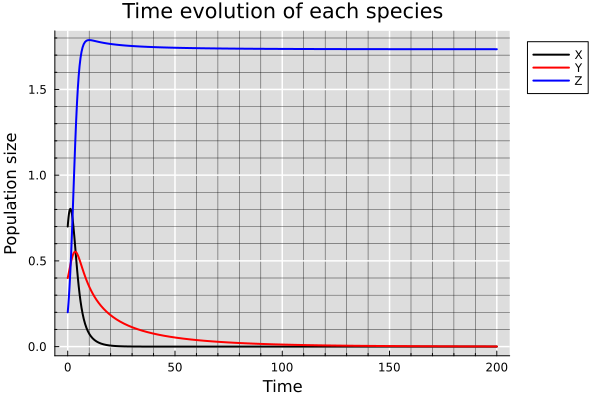
\includegraphics[width=\textwidth]{z_axial.png}
        \caption{$z$-axial equilibria; $r_1 = 0.404$, $r_2 = 0.903$, $p = 0.182$, $\gamma_{12} = 0.639$, $\gamma_{21} = 0.283$, $\gamma_{13} = 0.301$, $\gamma_{31} = 0.110$, $v_1 = 0.645$, $v_2 = 0.175$, $v_3 = 0.145$.}
        \label{fig:z_axial}
    \end{subfigure}
    \hfill
    \begin{subfigure}[b]{0.47\textwidth}
        \centering
        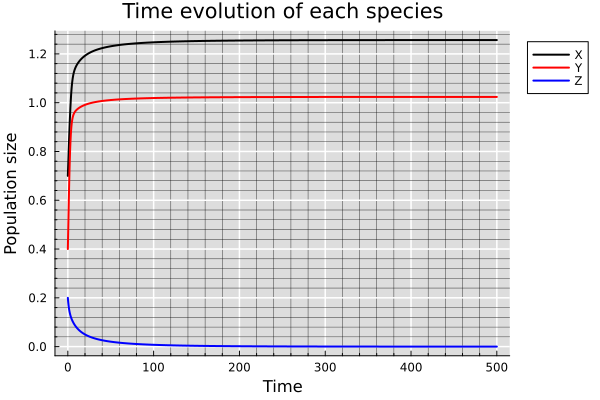
\includegraphics[width=\textwidth]{xy_boundary.png}
        \caption{$xy$-boundary equilibria; $r_1 = 0.978$, $r_2 = 0.613$, $p = 0.326$, $\gamma_{12} = 0.245$, $\gamma_{21} = 0.015$, $\gamma_{13} = 0.920$, $\gamma_{31} = 0.696$, $v_1 = 0.523$, $v_2 = 0.951$, $v_3 = 0.570$.}
        \label{fig:xy_boundary}
    \end{subfigure}
    \hfill
    \begin{subfigure}[b]{0.47\textwidth}
        \centering
        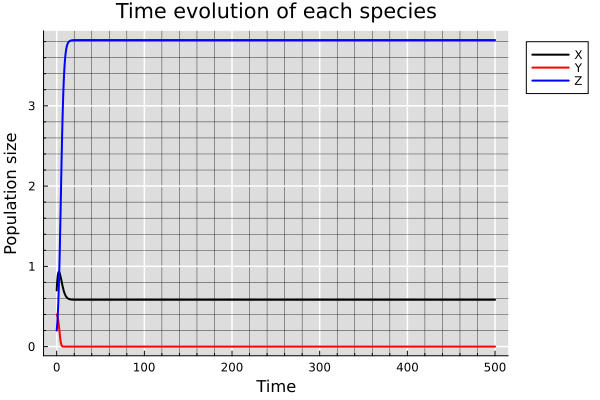
\includegraphics[width=\textwidth]{xz_boundary.png}
        \caption{$xz$-boundary equilibria; $r_1 = 0.102$, $r_2 = 0.763$, $p = 0.271$, $\gamma_{12} = 0.182$, $\gamma_{21} = 0.301$, $\gamma_{13} = 0.109$, $\gamma_{31} = 0.198$, $v_1 = 0.983$, $v_2 = 0.186$, $v_3 = 0.113$.}
        \label{fig:xz_boundary}
    \end{subfigure}
    \hfill
    \begin{subfigure}[b]{0.47\textwidth}
        \centering
        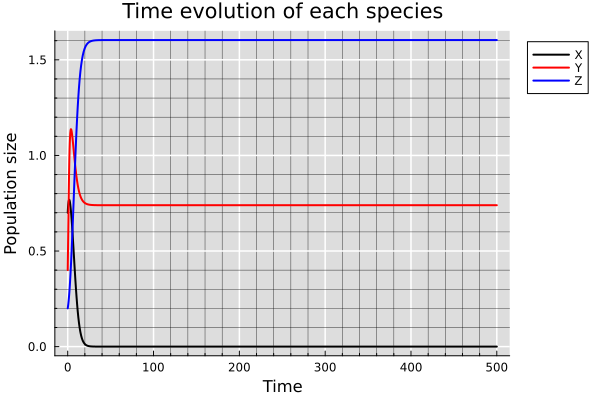
\includegraphics[width=\textwidth]{yz_boundary.png}
        \caption{$yz$-boundary equilibria; $r_1 = 0.978$, $r_2 = 0.310$, $p = 0.843$, $\gamma_{12} = 0.002$, $\gamma_{21} = 0.407$, $\gamma_{13} = 0.859$, $\gamma_{31} = 0.446$, $v_1 = 0.872$, $v_2 = 0.201$, $v_3 = 0.959$.}
        \label{fig:yz_boundary}
    \end{subfigure}
       \caption{Showing the stability of equilibrium points with different set of parameters.}
       \label{fig:semi-trivial-equilibria-plots}
\end{figure}

\begin{figure}[H]
    \centering
    \begin{subfigure}[b]{0.49\textwidth}
        \centering
        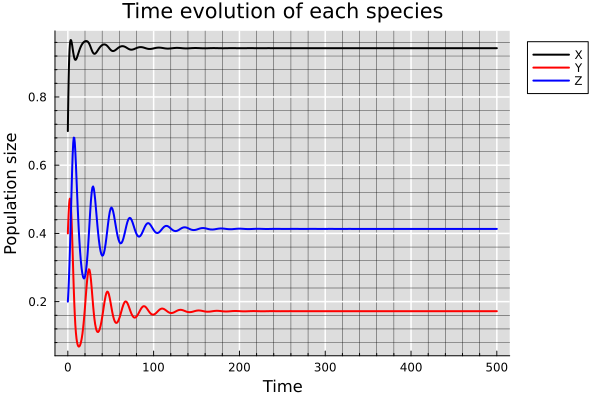
\includegraphics[width=\textwidth]{interior.png}
        \caption{Stability of the interior equilibrium.}
        \label{fig:interior}
    \end{subfigure}
    \hfill
    \begin{subfigure}[b]{0.49\textwidth}
        \centering
        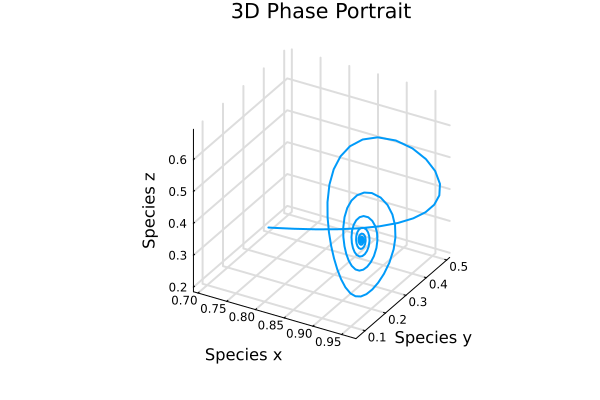
\includegraphics[width=\textwidth]{interior_pp_3D.png}
        \caption{3D phase portrait.}
        \label{fig:phase_plane_3d}
    \end{subfigure}
    \hfill
    \begin{subfigure}[b]{0.49\textwidth}
        \centering
        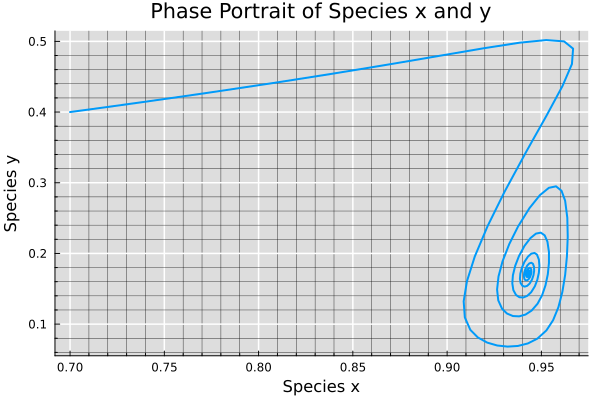
\includegraphics[width=\textwidth]{interior_pp_xy.png}
        \caption{$xy$ phase plane.}
        \label{fig:phase_plane_xy}
    \end{subfigure}
    \hfill
    \begin{subfigure}[b]{0.49\textwidth}
        \centering
        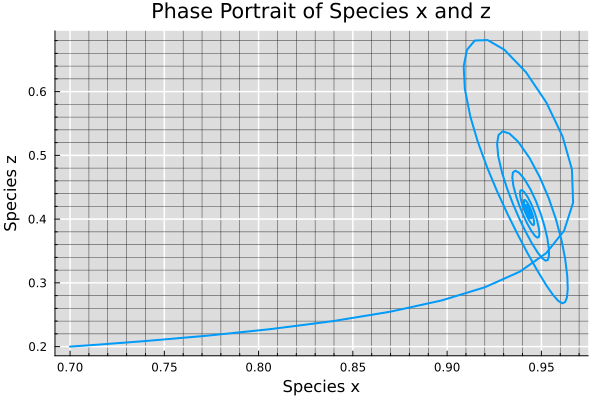
\includegraphics[width=\textwidth]{interior_pp_xz.png}
        \caption{$xz$ phase plane.}
        \label{fig:phase_plane_xz}
    \end{subfigure}
    \hfill
    \begin{subfigure}[b]{0.49\textwidth}
        \centering
        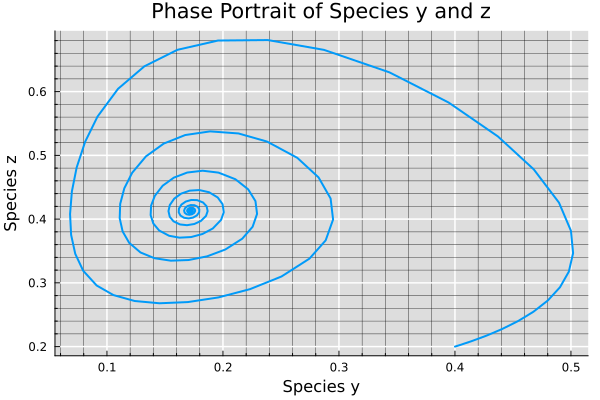
\includegraphics[width=\textwidth]{interior_pp_yz.png}
        \caption{$yz$ phase plane.}
        \label{fig:phase_plane_yz}
    \end{subfigure}
       \caption{Different types of plots to show the behavior of \myref[Model]{model:3.2} where $r_1 = 0.635$, $r_2 = 0.742$, $p = 0.853$, $\gamma_{12} = 0.142$, $\gamma_{21} = 0.002$, $\gamma_{13} = 0.148$, $\gamma_{31} = 0.215$, $v_1 = 0.090$, $v_2 = 0.891$, $v_3 = 0.980$.}
       \label{fig:nontrivial-equilibria-plots}
\end{figure}


\end{document}
